Recall that if \(R\) is a CU ring, we say that two elements \(a,b \in R\) are \emph{associate}, denoted \(a \ASSOC b\), if there is a unit \(u \in R\) such that \(a = ub\).
It turns out that the divisibility structure of \(R\) cannot distinguish associates from each other.
Considering associate elements to be ``the same'', we have a nice way to visualize the divisibility structure of a ring.

Recall that if \(\sigma\) is an equivalence relation on a set \(X\), then we have a canonical \emph{partition} of \(X\) induced by \(\sigma\) given by the \(\sigma\)-classes.
This partition, considered as a set, is called the \emph{quotient} of \(X\) by \(\sigma\), and acts very much like \(X\) does except that elements of \(X\) which are \(\sigma\) related become equal in \(X/\sigma\).
This is a powerful idea which we will use again in \autoref{chap:quot}.
For now, we will use the classes of the associate relation to reason about divisibility.

\begin{dfn}[Associate Structure] \label{dfn:assoc-sld}
Let \(R\) be a CU ring.
Recall by \eref{exerc:assoc-equiv} that \(\ASSOC\) is an equivalence relation on \(R\).
The set \(\ASSOCLAT{R} = R/\!\!\ASSOC\) of all \(\ASSOC\)-equivalence classes of \(R\) is called the \emph{associate structure} of \(R\).
\end{dfn}

Note that, by definition, the associate class of \(a\) is all the elements of the form \(ua\) where \(u\) is a unit.
If \(R\) is small enough we can find its associate classes by hand.
For example, the associate classes of \(\ZZ/(4)\) are \([0] = \{0\}\), \([1] = \{1,3\}\), and \([2] = \{2\}\).
The ring \(\ZZ\) is not very small, but we can see that its associate classes are \([0]\) and \([n] = \{ n, -n \}\) where \(n > 0\).
As promised, the divisibility relation on \(R\) can be bumped up to a kind of relation on \(\ASSOCLAT{R}\).

\begin{prop}
Let \(R\) be a CU ring.
We define a relation \(\lesssim\) on \(\ASSOCLAT{R}\) as follows: given two associate classes \(A\) and \(B\), we say \(A \lesssim B\) if there exist \(a \in A\) and \(b \in B\) such that \(a|b\).
Then the following hold for all \(A,B,C \in \ASSOCLAT{R}\).
\begin{proplist*}
\item If \(A \lesssim B\), then in fact \(a|b\) for \emph{any} \(a \in A\) and \(b \in B\).
\item \(A \lesssim A\).
\item If \(A \lesssim B\) and \(B \lesssim C\), then \(A \lesssim C\).
\item If \(R\) is a domain, then if \(A \lesssim B\) and \(B \lesssim A\) then \(A = B\).
\end{proplist*}
\end{prop}

\begin{proof}
\begin{inlineproplist}
\item Since \(A \lesssim B\), there exist \(x \in A\) and \(y \in B\) such that \(x|y\).
Now \(a \ASSOC x\) and \(b \ASSOC y\), so using \eref{exerc:associate-divides}, we have \(x|y\) if and only if \(x|b\), if and only if \(a|b\).
\item Let \(a \in A\); now \(a|a\) as needed.
\item Let \(a \in A\), \(b \in B\), and \(c \in C\).
We have \(a|b\) and \(b|c\), so that \(a|c\).
\item Let \(a \in A\) and \(b \in B\).
We have \(a|b\) and \(b|a\); say \(b = xa\) and \(a = yb\).
Substituting, we have \(1_rb = b = xyb\); by cancellation, \(xy = 1_R\), and thus \(x\) and \(y\) are units as needed.
\end{inlineproplist}
\end{proof}

For any ring \(R\) the \(\lesssim\) relation is both reflexive and transitive.
Such relations are sometimes called \emph{preorders}, and can be visualized using a kind of picture called a \emph{Hasse diagram}\index{Hasse diagram}.
To draw the Hasse diagram of a preorder like \(\ASSOCLAT{R}\), we draw each element on the page so that if \(A \lesssim B\) then \(A\) is \emph{below} \(B\).
Then we connect \(A\) and \(B\) by a line if and only if there are no other elements \(C\) such that \(A \lesssim C \lesssim B\).
In the special case that \(A\) and \(B\) are distinct but \(A \lesssim B\) and \(B \lesssim A\), we simply write \(A\) and \(B\) adjacent to each other.
We call the Hasse diagram of \(\ASSOCLAT{R}\) the \emph{divisor diagram}\index{divisor diagram} of \(R\).

As an example, consider the ring \(\ZZ/(12)\).
The associate classes of this ring are \([0] = \{0\}\), \([1] = \{1,5,7,11\}\), \([2] = \{2,10\}\), \([3] = \{3,9\}\), \([4] = \{4,8\}\), and \([6] = \{6\}\); the divisor diagrams of \(\ZZ/(12)\) and two other rings are shown in Figure \ref{fig:divisor-diagrams}.

\begin{figure}[h!]
\begin{center}
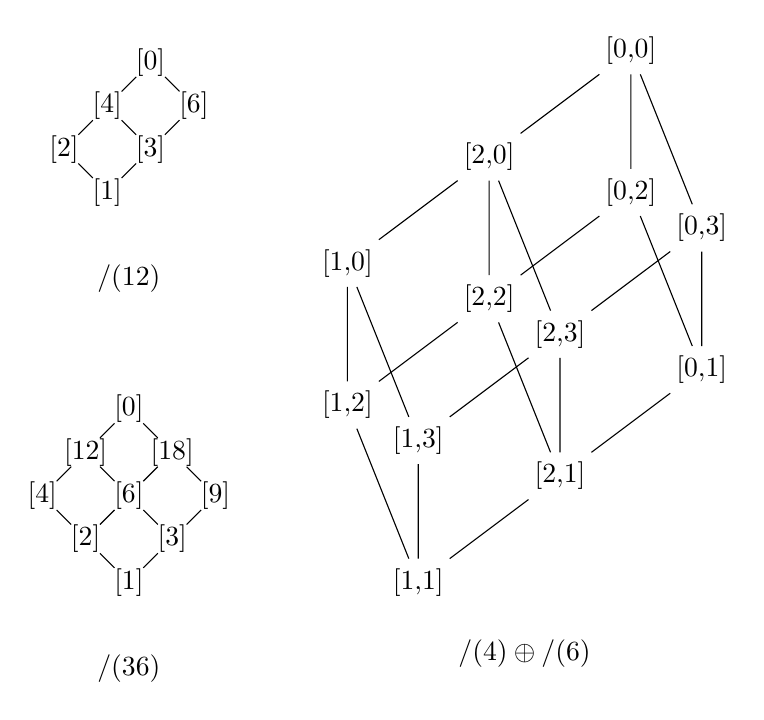
\begin{tikzpicture}
  \begin{scope}[scale=0.55,shift={(0,9)},vtx/.style={inner sep=0}]
    \node[vtx,align=center] (1) at (1,0) {\([1]\)};
    \node[vtx,align=center] (2) at (0,1) {\([2]\)};
    \node[vtx,align=center] (3) at (2,1) {\([3]\)};
    \node[vtx,align=center] (4) at (1,2) {\([4]\)};
    \node[vtx,align=center] (6) at (3,2) {\([6]\)};
    \node[vtx,align=center] (0) at (2,3) {\([0]\)};
    \draw[-] (1) -- (2) -- (4) -- (0) -- (6) -- (3) -- (4);
    \draw[-] (1) -- (3);
    \node (label) at (1.5,-2) {\(\ZZ/(12)\)};
  \end{scope}

  \begin{scope}[scale=0.55,shift={(0.5,0)},vtx/.style={inner sep=0}]
    \node[vtx,align=center] (1)  at (1,0) {\([1]\)};
    \node[vtx,align=center] (2)  at (0,1) {\([2]\)};
    \node[vtx,align=center] (3)  at (2,1) {\([3]\)}; 
    \node[vtx,align=center] (4)  at (-1,2) {\([4]\)};
    \node[vtx,align=center] (6)  at (1,2)  {\([6]\)};
    \node[vtx,align=center] (9)  at (3,2)  {\([9]\)};
    \node[vtx,align=center] (12) at (0,3) {\([12]\)};
    \node[vtx,align=center] (18) at (2,3) {\([18]\)};
    \node[vtx,align=center] (0)  at (1,4) {\([0]\)};
    \draw[-] (1) -- (2) -- (4) -- (12) -- (0) -- (18) -- (6) -- (12);
    \draw[-] (18) -- (9) -- (3) -- (6) -- (2);
    \draw[-] (1) -- (3);
    \node[align=center] (label) at (1,-2) {\(\ZZ/(36)\)};
  \end{scope}

  \begin{scope}[scale=0.45,shift={(8,0)}]
    \coordinate (O) at (0,0);
    \node[align=center] (11) at (2,0)   {\([1,\!1]\)};
    \node[align=center] (12) at (0,5)   {\([1,\!2]\)};
    \node[align=center] (13) at (2,4)   {\([1,\!3]\)};
    \node[align=center] (10) at (0,9)   {\([1,\!0]\)};
    \node[align=center] (21) at (6,3)   {\([2,\!1]\)};
    \node[align=center] (22) at (4,8)   {\([2,\!2]\)};
    \node[align=center] (23) at (6,7)   {\([2,\!3]\)};
    \node[align=center] (20) at (4,12)  {\([2,\!0]\)};
    \node[align=center] (01) at (10,6)  {\([0,\!1]\)};
    \node[align=center] (02) at (8,11)  {\([0,\!2]\)};
    \node[align=center] (03) at (10,10) {\([0,\!3]\)};
    \node[align=center] (00) at (8,15)  {\([0,\!0]\)};
    \draw[-] (11) -- (12) -- (10) -- (13) -- (11);
    \draw[-] (21) -- (22) -- (20) -- (23) -- (21);
    \draw[-] (01) -- (02) -- (00) -- (03) -- (01);
    \draw[-] (11) -- (21) -- (01);
    \draw[-] (12) -- (22) -- (02);
    \draw[-] (13) -- (23) -- (03);
    \draw[-] (10) -- (20) -- (00);
    \node[align=center] (label) at (5,-2) {\(\ZZ/(4) \oplus \ZZ/(6)\)};
  \end{scope}
\end{tikzpicture}
\end{center}
\caption{\label{fig:divisor-diagrams} Some divisor diagrams.}
\end{figure}

Even if the divisor diagram of \(R\) is infinite it may be helpful to see small parts of it at a time.
If \(a \in R\) is an element, the divisor diagram of \(a\) in \(R\) is simply the hasse diagram of the divisors of \(a\).
Divisor diagrams provide an important answer to what we might call the Visualization Problem.
\begin{titlebox}{The Visualization Problem}
\begin{center}
Given a ring, can we draw a picture of it?
\end{center}
\end{titlebox}
In addition to divisor diagrams both cayley tables and commutative diagrams are also useful visualization tools, and we will see others.
For infinite rings, or even just large finite rings, the complete divisor diagram may not be very helpful.
But even just looking at a portion of the diagram can give insight.
Seeing a ring in this way can also lead us to make conjectures.
For instance, perhaps \(R\) is infinite, but \(\ASSOCLAT{R}\) is finite, or has only finite ``height'', or ``width'' (whatever that means), or has only finitely many minimal or maximal elements.
Does that imply anything about \(R\)?
Do divisor diagrams always have the boxy shape of the examples in Figure \ref{fig:divisor-diagrams}?



%---------%
\Exercises%
%---------%

\begin{exercise}
Compute the associate classes of \(\ZZ\).
\end{exercise}


\begin{exercise}
Draw the divisor diagrams of the following rings.
\begin{proplist*}
\item \(\ZZ/(8)\)
\item \(\POW{\{a,b,c\}}\)
\item \(\ZZ/(4) \oplus \ZZ/(4)\)
\item \(\ZZ/(36)\)
\end{proplist*}
\end{exercise}


\begin{exercise}
Show that \(R\) is a field precisely when \(\ASSOCLAT{R}\) consists only of \([0]\) and \([1]\).
\end{exercise}


\begin{exercise}
(@@@) find a CU nondomain and \(a\), \(b\) where \(a|b\) and \(b|a\) but \(a\), \(b\) not associate.
\end{exercise}


\begin{exercise}
Show that divisibility on \(\ZZ/(4)\) is symmetric.
\end{exercise}


\begin{exercise}
Let \(R\) be a domain.
Show that \(a \in R\) is irreducible if and only if \([a]\) is \(\lesssim\)-minimal.
\end{exercise}


\begin{exercise} \label{exerc:assoc-prod}
Let \(R\) be a CU ring.
We define a kind of setwise product on associate classes as follows: given \(A,B \in \ASSOCLAT{R}\), we define \[ A \ast B = \{ ab \mid a \in A, b \in B \}. \]
Show that the following hold.
\begin{proplist*}
\item \(A \ast B \in \ASSOCLAT{R}\), so that \(\ast\) is a binary operation on \(\ASSOCLAT{R}\).
\item \((A \ast B) \ast C = A \ast (B \ast C)\) for all \(A,B,C \in \ASSOCLAT{C}\).
\item \(A \ast B = B \ast A\) for all \(A,B \in \ASSOCLAT{R}\).
\item \label{exerc:assoc-prod:cancel} If \(R\) is a domain and \(A \ast C = B \ast C\), then \(A = B\).
\end{proplist*}
\end{exercise}


\begin{dfn}[Monotone Map]
Recall that a \emph{preorder} is a set \(P\) equipped with a relation \(\lesssim\) which is reflexive and transitive.
If \(P\) and \(Q\) are preorders, a mapping \(\varphi : P \rightarrow Q\) is called \emph{monotone}\index{monotone} if whenever \(a \lesssim b\) in \(P\) we have \(\varphi(a) \lesssim \varphi(b)\) in \(Q\).
Similarly, we say \(\varphi\) is \emph{antitone} if whenever \(a \lesssim b\) in \(P\) we have \(\varphi(b) \lesssim \varphi(a)\) in \(Q\).
\end{dfn}


\begin{exercise}
Let \(R\) be a CU ring.
\begin{proplist*}
\item Show that \(R\) is a preorder under the divisibility relation.
\item Show that the mapping \(\varphi : R \rightarrow \ASSOCLAT{R}\) given by \(\varphi(r) = [r]\) is a preorder homomorphism.
\end{proplist*}
\end{exercise}


\begin{exercise}
Let \(\varphi : R \rightarrow S\) be a ring homomorphism, where \(R\) and \(S\) are commutative.
Show that, if we consider \(R\) and \(S\) to be preorders under divisibility, then \(\varphi\) is monotone.
\end{exercise}


\begin{exercise}
Let \(\varphi : R \rightarrow S\) be a unital ring homomorphism.
\begin{proplist}
\item Show that if \(a,b \in R\) and \(a \ASSOC b\), then \(\varphi(a) \ASSOC \varphi(b)\).
\item Show that the relation \( \Phi \subseteq \ASSOCLAT{R} \times \ASSOCLAT{S} \) given by \[ \Phi = \{ ([a],[\varphi(a)]) \mid a \in R \} \] is well-defined and total.
\item Show that \(\Phi\) is monotone.
\item Show that if \(\varphi\) is surjective, then \(\Phi\) is surjective.
\end{proplist}
\end{exercise}
